

\begin{flushleft}

	
	Converting one primitive data type into another is known as type conversion. There are two types of type conversions:

	
	\begin{itemize}

		\item \textbf{Implicit type casting or widening:} 
		\begin{itemize}
			\item \textbf{Converting a lower datatype to a higher datatype} is known as widening or up-casting.
			\item Compiler is responsible to perform implicity type casting.
			\item There is no loss of information in this type casting.
			\item The following are various possible conversions:
		\end{itemize}
		

		
		\begin{figure}[h!]
			\centering
			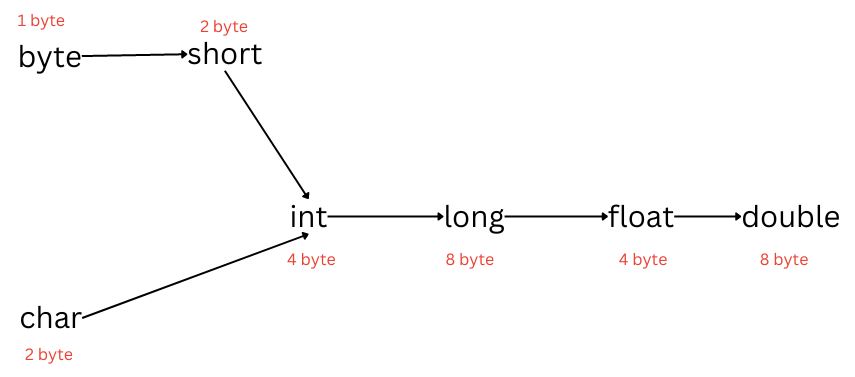
\includegraphics[scale=.4]{content/chapter2/images/convert.png}

		\end{figure}		
		Eg:
		\codeblock{
			int x = 'a';  \\
			System.out.println(x);    // output: 97 \\
			\\
			double d = 10; \\
			System.out.println(d);  // output: 10.0
		}
	
		\bigskip
		\noteblock{
			\begin{itemize}
				\item \textbf{Long value can be assigned to float variable} because both are following different memory representations internally. 
			\end{itemize}
		}
		
		
		\newpage
		
		\item \textbf{Explicit type casting or narrowing:} 
		\begin{itemize}
			\item Converting a higher datatype to a lower datatype is known as narrowing or down casting.
			\item Programmer is responsible to perform explicit type casting.
			\item Loss of information is possible.
			\item The following are various possible conversions:
			
			\newimage{0.35}{content/chapter2/images/rev.png}
			
			\item Except for boolean, all datatypes can be type-cast to other primitive data-type.
			\item Type-cast operator for each primitive datatype:
			
		\end{itemize}
		
		\tablethree{
			\hline
			Data type & Type-case operator & Example \\
			\hline
			byte & (byte) &  double d = 130.4; \newline byte x = (byte) d; \\
			\hline
			short & (short) & double d = 130.4; \newline short x = (short) d; \\
			\hline
			int & (int) & double d = 130.4; \newline int x = (int) d; \\
			\hline
			long & (long) & double d = 130.4; \newline long x = (long) d; \\
			\hline
			float & (float) & double d = 130.4; \newline float x = (float) d; \\
			\hline
			double & (double) & float d = 130.4; \newline double x = (double) d; \\
			\hline
			char & (char) & double d = 130.4; \newline char x = (char) d; \\
			\hline
		}
		\newpage
		Eg 1:
		\codeblock{
			int x = 130; \\
			//byte b = x;      \xmark \\
			byte b = (byte) x;  \cmark    \\
			System.out.println(b);   // output: -126
		}
	
		Output explaination:
		\begin{itemize}
			\item Integer is 32-bit in size \& byte is 8-bit in size.
			\item 32-bit binary representation of 130 is 0000000…10000010.
			\item To convert integer to byte datatype, mean downsize decimal representation of 130 to fit in 8 bit.
			\item Which means the binary number \textbf{0000000…10000010} is down-sized to \textbf{10000010}
			\item Note that left-most bit is "1" and hence number is now represented as 2's complement.
			\item 2's complement of \textbf{10000010} is \textbf{11111101+1 => 11111110 => -126}
		\end{itemize}

		\bigskip

		Eg 2: If we assign floating point values to integral types, by explicit type casting, the digits after decimal point will be lost.
		\bigskip
		\codeblock{
			double d = 130.456; \\
			int x = (int) d;  \\
			System.out.println(x); // output: 130 \\
			\\
			byte b = (byte) d;  \\
			System.out.println(b);  // output: -126
		}
		
	\end{itemize}
	
\end{flushleft}

